\clearpage
%//==============================--@--==============================//%
\subsection[4.4 Data Plane]{\hspace*{0.075 em}\raisebox{0.2 em}{$\pmb{\drsh}$} Data Plane}
\label{subsec:data-plane}

%//==============================--@--==============================//%
\subsubsection[4.4.1 IPv4 Datagram Format]{$\rightarrow$ IPv4 Datagram Format}

\vspace{-0.5em}
\begin{figure}[H]
    \centering
    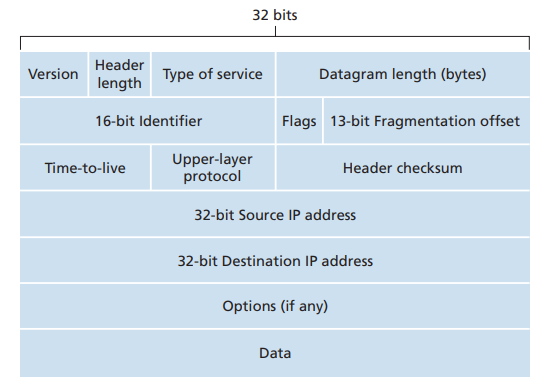
\includegraphics[width = 0.7\linewidth]{img/4/data-plane/IPv4-datagram-format.png}
    \caption{IPv4 Datagram format \cite{Kurose2017}}
    \label{fig:IPv4}
\end{figure}

\begin{itemize}
    \item \textbf{Version number (4 bits):} Specifies the IP protocol version of the datagram, e.g., IPv4 or IPv6.
    
    \item \textbf{Header length (4 bits):} Indicates where the payload begins, considering variable number of options in the header.
    
    \item \textbf{Type of service (8 bits):} Distinguishes different types of IP datagrams, e.g., real-time vs non-real-time traffic, and supports Explicit Congestion Notification.
    
    \item \textbf{Datagram length (16 bits):} Total length of the IP datagram (header plus data) in bytes, with a theoretical maximum size of 65,535 bytes.
    
    \item \textbf{Identifier, flags, fragmentation offset (32 bits):} Related to IP fragmentation, where large datagrams are split into smaller ones, then reassembled at the destination.
    
    \item \textbf{Time-to-live (8 bits):} Ensures datagrams don't circulate indefinitely; decre- mented by one at each router, and dropped when reaching zero.
    
    \item \textbf{Protocol (8 bits):} Indicates the transport-layer protocol for the payload (e.g., 6 for TCP, 17 for UDP).
    
    \item \textbf{Header checksum (16 bits):} Helps detect bit errors in the received IP datagram using 1s complement arithmetic; recomputed and stored at each router.
    
    \item \textbf{Source IP address (32 bits):} IP address of the sender.
    
    \item \textbf{Destination IP address (32 bits):} IP address of the intended recipient.
    
    \item \textbf{Options (variable):} Allow IP header to be extended; used rarely and not included in IPv6 header.
    
    \item \textbf{Data (payload):} Contains the transport-layer segment (e.g., TCP or UDP) or other data types (e.g., ICMP messages) to be delivered to the destination.
\end{itemize}

%//==============================--@--==============================//%
\subsubsection[4.4.2 IPv4 Addressing]{$\rightarrow$ IPv4 Addressing}

\noindent Each IP address is 32 bits long (equivalently, 4 bytes). These addresses are typically written in so-called dotted-decimal notation, in which each byte of the address is written in its decimal form and is separated by a period (dot) from other bytes in the address:
$$
    \texttt{193.32.216.9} \pmb{\rightarrow} \texttt{11000001 00100000 11011000 00001001}
$$

\paragraph[4.4.2.1 Subnet and CIDR]{$\pmb{\star}$ Subnet and CIDR}\mbox{}
\begin{theo}[\underline{Subnet}]{def:Subnet}\label{def:Subnet}
    ``To determine the subnets, detach each interface from its host or router, creating islands of isolated networks, with interfaces terminating the end points of the isolated networks. Each of these isolated networks is called a subnet."\cite{Kurose2017}
\end{theo}

\vspace{-0.5em}
\begin{figure}[H]
    \centering
    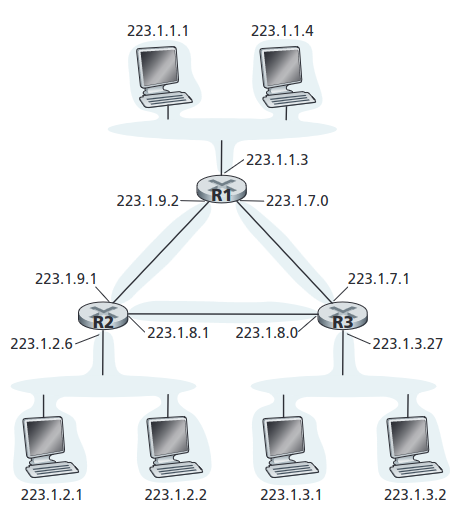
\includegraphics[width = 0.5\linewidth]{img/4/data-plane/Subnets}
    \caption{3 routers connected to 6 subnets}
    \label{fig:Subnet}
\end{figure}

\begin{itemize}[noitemsep, nolistsep]
    \item The boundary between the host and the physical link is called an \textbf{interface}. A router may have more than one interface (In \hyperref[fig:Subnet]{Fig. 39} each of the three routers possess 3 different interfaces)
    
    \item Multiple subnets can exist in a network, including point-to-point links connecting routers (see \hyperref[fig:Subnet]{Fig. 39}).
    
    \item An organization's network devices typically have IP addresses with a common network prefix.
    
    \item \textbf{Classless Interdomain Routing (CIDR)} generalizes subnet addressing by dividing the 32-bit IP address into two parts, with the network prefix indicated by x (\textbf{subnet mask}) in the a.b.c.d/x format (e.g.: \texttt{223.3.2.1/24} has prefix \texttt{223.3.2}).

    \item The x most significant bits are the network prefix, while the remaining 32-x bits can be used for subnetting within the organization.
\end{itemize}

\vspace{1 em}
\noindent\textbf{Nota:}\\
Address \texttt{255.255.255.255} is known has a brodcast address and is used to deliver a message to all hosts in the same subnet.

\paragraph[4.4.2.2 Allocating a block of addresses ]{$\pmb{\star}$ Allocating a block of addresses}\mbox{}
\begin{itemize}
    \item Network administrators obtain IP address blocks for their organizations from ISPs.
    
    \item ISPs can divide a larger allocated block into smaller blocks for their customers (e.g.: ISP's block \texttt{200.23.16.0/20} can be divided into eight smaller blocks for organizations such as \texttt{200.23.16.0/23}, \texttt{200.23.18.0/23} and so on).
    
    \item ISPs and other organizations can also obtain IP address blocks from a global authority, the \textbf{Internet Corporation for Assigned Names and Numbers (ICANN)}.
    
    \item ICANN manages IP addresses, DNS root servers, domain names, and domain name disputes, and allocates addresses to regional Internet registries.
\end{itemize}

%//==============================--@--==============================//%
\subsubsection[4.4.3 The Dynamic Host Configuration Protocol (DHCP)]{$\rightarrow$ The Dynamic Host Configuration Protocol (DHCP)}

\begin{itemize}
    \item Dynamic Host Configuration Protocol (DHCP) automates IP address assignment for hosts.
    \item Provides plug-and-play or zero-configuration functionality.
    \item Widely used in residential, enterprise, and wireless networks.
    \item DHCP operates as a client-server protocol.
    \item If no server is present on a subnet, a DHCP relay agent (typically a router) is needed.
\end{itemize}

\begin{figure}[H]
    \centering
    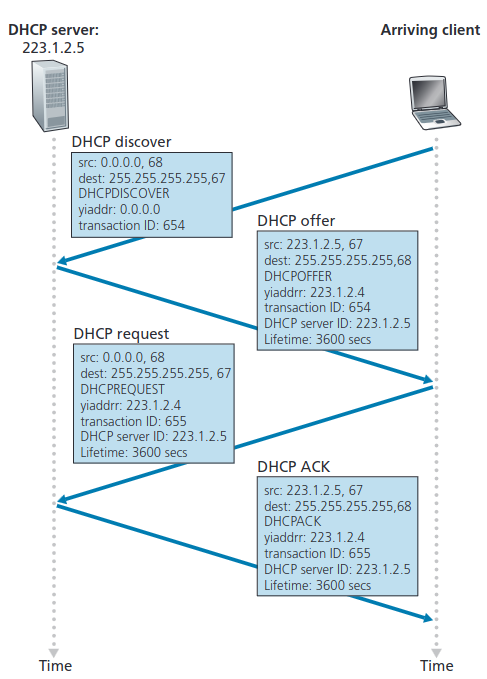
\includegraphics[width = 0.6\linewidth]{img/4/data-plane/DHCP.png}
    \caption{Client-server DHCP protocol}
    \label{fig:DHCP}
    \end{figure}

\begin{enumerate}[nolistsep]
    \item \textbf{DHCP server discovery:} Client sends a DHCP discover message using the broadcast destination IP address \texttt{255.255.255.255} and source IP address \texttt{0.0.0.0.}
    
    \item \textbf{DHCP server offer(s):} DHCP server responds with a DHCP offer message, also broadcast to all nodes on the subnet. Offer message contains transaction ID, proposed IP address, network mask, and IP address lease time.
    
    \item \textbf{DHCP request:} Client chooses an offer and responds with a DHCP request message, echoing back the configuration parameters (usually DHCP request is broadcasted, however, the client can choose to unicast it directly to the DHCP server if the server's IP address is known, the same can be said for DHCP ACK).
    
    \item \textbf{DHCP ACK:} Server responds with a DHCP ACK message, confirming the requested parameters.
\end{enumerate}

%//==============================--@--==============================//%
\subsubsection[4.4.4 Network Address Translation (NAT)]{$\rightarrow$ Network Address Translation (NAT)}

\begin{figure}[H]
    \centering
    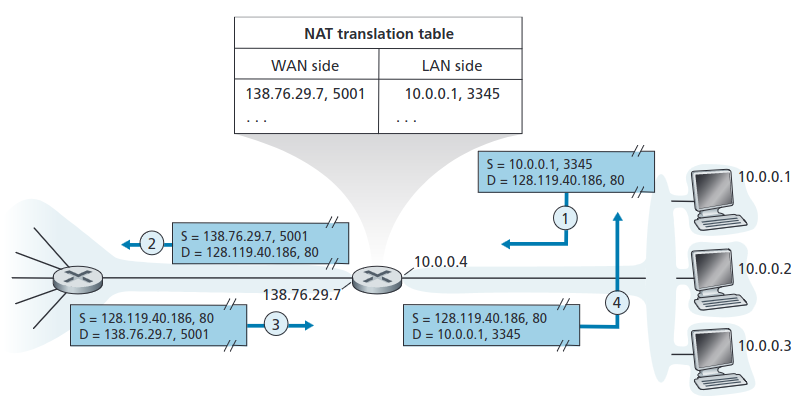
\includegraphics[width = 0.9\linewidth]{img/4/data-plane/NAT.png}
    \caption{Network address translation}
    \label{fig:NAT}
\end{figure}

\noindent The NAT-enabled router does not look like a router to the outside world. Instead
the NAT router behaves to the outside world as a single device with a single IP
address, possessing a \textbf{NAT translation table} capable of redirecting any messages to their specified destination through an (IP, PORT) association:

\begin{enumerate}
    \item User requests a Web page from a Web server (port 80) with IP address \texttt{128.119.40.186}.
    \item Host \texttt{10.0.0.1} assigns source port number 3345 and sends the datagram into the LAN.
    \item NAT router generates a new source port number 5001, replaces the source IP address and port, and adds an entry to its NAT translation table.
    \item Web server responds with a datagram \textbf{whose destination address is the NAT router's IP address}, and \textbf{destination port number is 5001}.
    \item NAT router uses the NAT translation table to obtain the appropriate IP address and destination port number for the browser in the home network, rewrites the datagram's destination address and port, and forwards the datagram into the home network.
\end{enumerate}

%//==============================--@--==============================//%
\clearpage
\subsubsection[4.4.5 IPv6 Datagram Format]{$\rightarrow$ IPv6 Datagram Format}

In the early 1990s, the Internet Engineering Task Force (IETF) began developing a successor to the IPv4 protocol due to concerns that the 32-bit IPv4 address space was running out. This led to the creation of the IPv6 protocol, which aimed to address the limitations of IPv4 and introduce improvements based on accumulated operational experience.

\begin{mdframed}
    \begin{itemize}[nolistsep, noitemsep]
        \item \textbf{IPv6 Address Representation:}
        \begin{itemize}[nolistsep, noitemsep]
            \item IPv6 addresses are 128 bits long, separated into 8 fields of 16 bits each.
            \item Each 16-bit field is represented by 4 hexadecimal characters.
        \end{itemize}
        \item Example:
        \begin{itemize}[nolistsep, noitemsep]
            \item Original: \texttt{2001:0db8:130f:0000:0000:7000:0000:140b}
            \item Simplified (without leading zeros): \texttt{2001:db8:130f:0:0:7000:0:140b}
            \item Further simplified (with consecutive zero fields replaced by "\texttt{::}"): \texttt{2001:db8:130f::7000:0:140b}
        \end{itemize}
    \end{itemize}
\end{mdframed}

\vspace{-0.5em}
\begin{figure}[H]
    \centering
    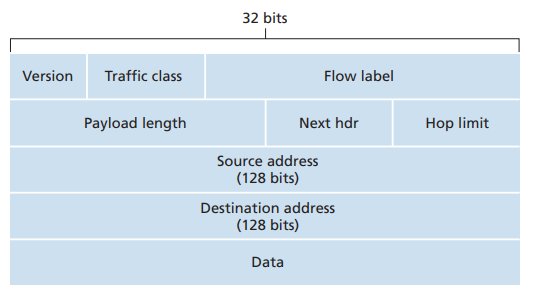
\includegraphics[width = 0.7\linewidth]{img/4/data-plane/IPv6-datagram-format.png}
    \caption{IPv6 Datagram format \cite{Kurose2017}}
    \label{fig:IPv6}
\end{figure}

\begin{itemize}
    \item \textbf{Version (4 bits):} Identifies the IP version number; IPv6 carries a value of 6.
    
    \item \textbf{Traffic class (8 bits):} Prioritizes certain datagrams within a flow or from specific applications, similar to the Type of Service in IPv4.
    
    \item \textbf{Flow label (20 bits):} Used to identify a flow of datagrams, with an elusive definition; could distinguish traffic from different applications or users.
    
    \item \textbf{Payload length (16 bits):} Unsigned integer giving the number of bytes in the IPv6 datagram following the fixed-length, 40-byte datagram header.
    
    \item \textbf{Next header (8 bits):} Identifies the protocol to which the data field of the datagram will be delivered (e.g., TCP, UDP); same values as IPv4 protocol field.
    
    \item \textbf{Hop limit (8 bits):} Contents decremented by one at each router; if the count reaches zero, the router discards the datagram.
    
    \item \textbf{Source address (128 bits):} IPv6 address of the sender, described in RFC 4291.
    
    \item \textbf{Destination address (128 bits):} IPv6 address of the intended recipient, described in RFC 4291.
    
    \item \textbf{Data (payload):} Transport-layer segment (e.g., TCP, UDP) or other data types (e.g., ICMP messages) to be delivered to the destination.
\end{itemize}

\noindent IPv6 also omits certain fields that were present in the IPv4 datagram format:
\begin{itemize}
    \item \textbf{Fragmentation/reassembly:} IPv6 does not allow fragmentation and reassembly at intermediate routers. If an IPv6 datagram is too large to be forwarded, the router drops the datagram and sends a "Packet Too Big" ICMP error message back to the sender, who can then resend the data using a smaller IP datagram size.

    \item \textbf{Header checksum:} Due to checksumming already being performed at the transport layer and link layer in the Internet, the header checksum was considered redundant and removed to speed up IP packet processing.

    \item \textbf{Options:} The options field is no longer a part of the standard IP header. Instead, it can be one of the possible next headers pointed to from within the IPv6 header, alongside TCP or UDP protocol headers. This change results in a fixed-length, 40-byte IP header.
\end{itemize}

\paragraph[4.4.5.1 Transitioning from IPv4 to IPv6]{$\pmb{\star}$ Transitioning from IPv4 to IPv6}\mbox{}

\begin{itemize}
    \item New IPv6 systems can be made backward-compatible, but deployed IPv4 systems cannot handle IPv6 datagrams.
    \item A "flag day" for simultaneous transition from IPv4 to IPv6 is not feasible due to the vast number of devices.
\end{itemize}

\begin{theo}[\underline{Tunneling}]{def:tunneling}\label{def:tunneling}
    \begin{itemize}[nolistsep,noitemsep]
        \item The most widely adopted approach for IPv4-to-IPv6 transition.
        \item IPv6 nodes wanting to communicate are connected by intervening IPv4 routers (forming a tunnel).
        \item The IPv6 node on the sending side encapsulates the entire IPv6 datagram into the payload field of an IPv4 datagram using the IPv6 protocol (number 41).
        \item The IPv4 routers in the tunnel route the IPv4 datagram without knowing it contains an IPv6 datagram, only aware of the IPv4 header information.
        \item The IPv6 node on the receiving side extracts the IPv6 datagram from the IPv4 datagram by recognizing protocol number 41 and routes it accordingly.
    \end{itemize}
\end{theo}

\begin{figure}[H]
    \centering
    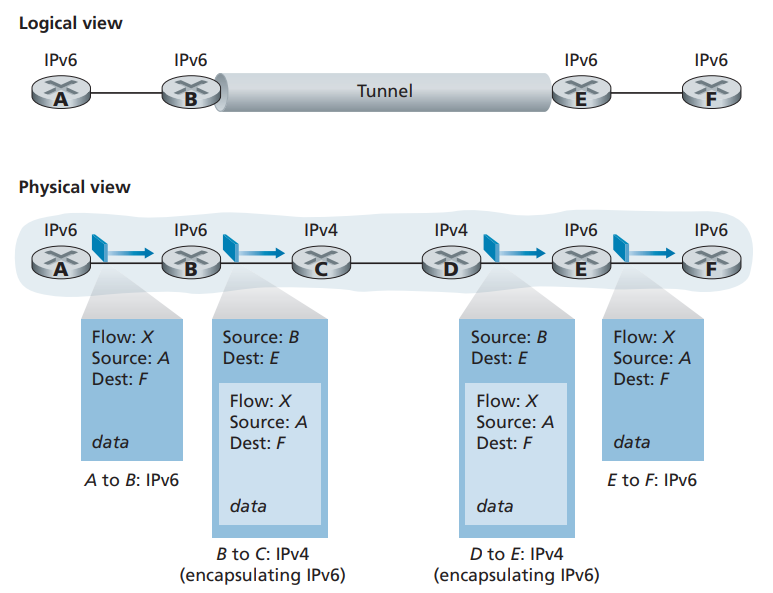
\includegraphics[width = 0.65\linewidth]{img/4/data-plane/tunneling.png}
    \caption{Tunneling \cite{Kurose2017}}
    \label{fig:tunneling}
\end{figure}

\newpage
\subsubsection[4.4.6 ICMP: The Internet Control Message Protocol]{$\rightarrow$ ICMP: The Internet Control Message Protocol}
\begin{theo}[\underline{ICMP}]{def:ICMP}\label{def:ICMP}
    ICMP is often considered part of IP, but architecturally it lies just above IP, as ICMP messages are carried inside IP datagrams. That is, ICMP messages are carried as IP payload, just as TCP or UDP segments are carried as IP payload. Similarly, when a host receives an IP datagram with ICMP specified as the upper-layer protocol (an upper-layer protocol number of 1), it demultiplexes the datagram’s contents to ICMP, just as it would demultiplex a datagram’s content to TCP or UDP.
\end{theo}

\noindent ICMP messages consist of \textbf{type} and \textbf{code fields} and contains the \textbf{header of first 8 bytes of the triggering IP datagram}. ICMP messages are not only for error signaling; the ping program sends an ICMP echo request and the destination host responds with an ICMP echo reply. Traceroute is implemented with ICMP messages, sending a series of IP datagrams with increasing TTL values to identify routers and round-trip times between the source and destination hosts. ICMPv6 has reorganized the existing ICMP types and codes and added new ones for IPv6 functionality.

\begin{figure}[H]
    \centering
    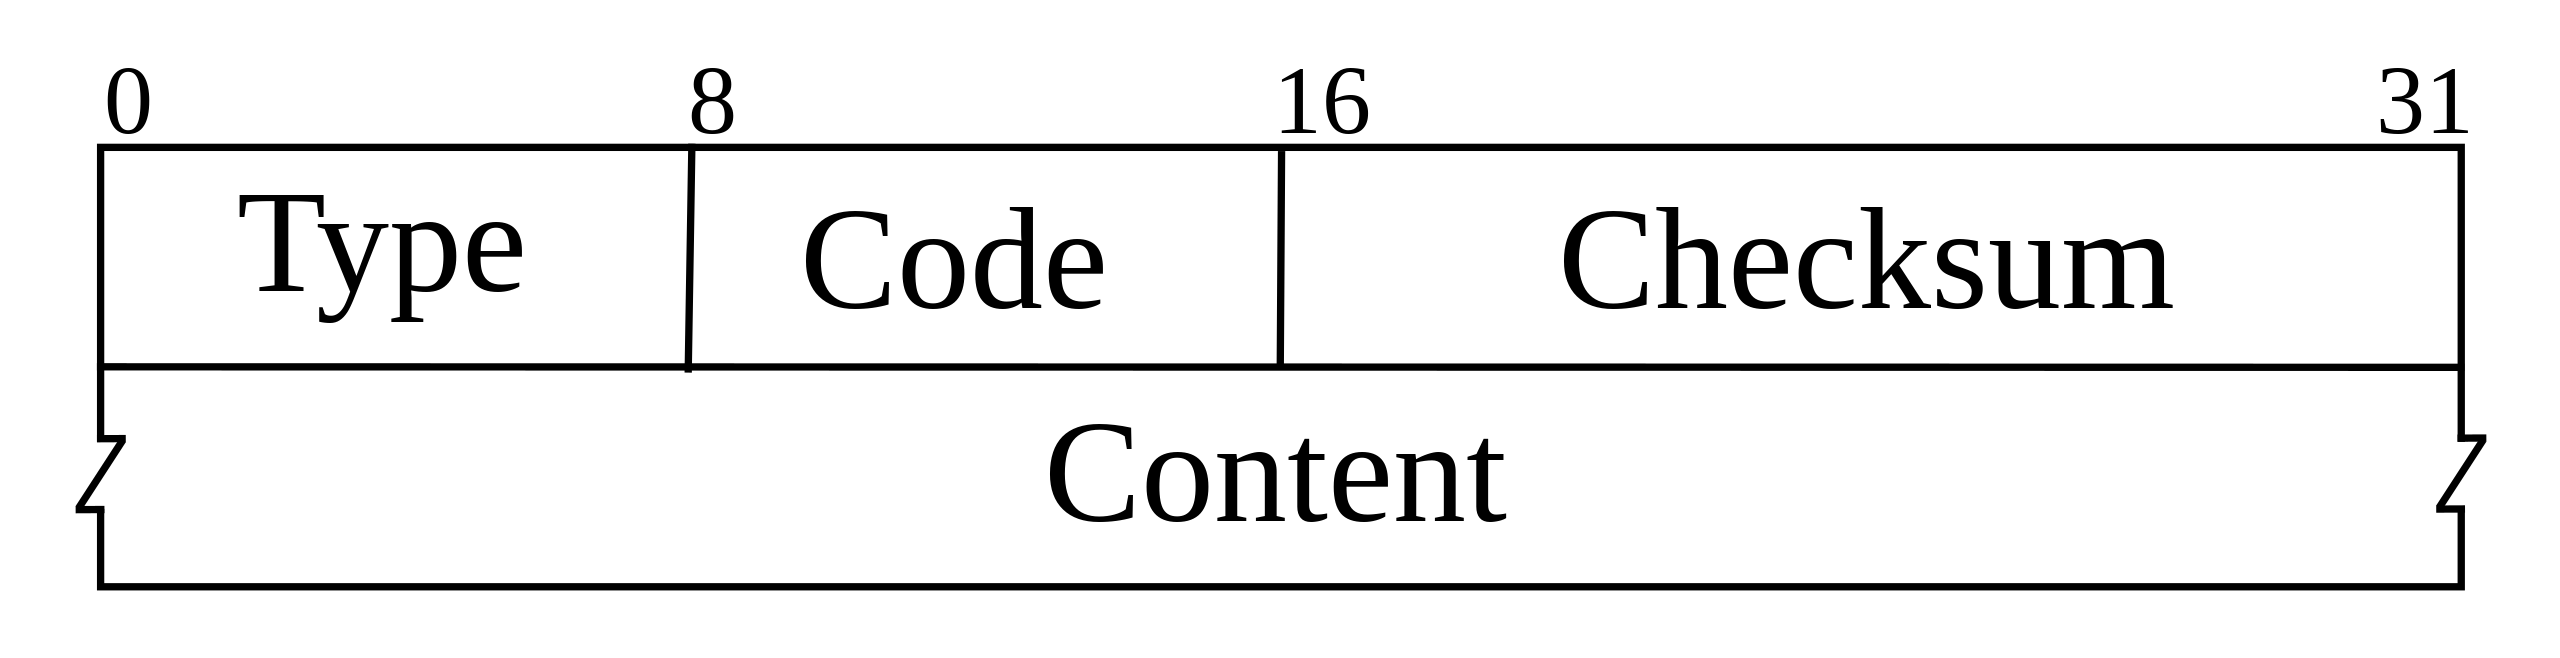
\includegraphics[width = 0.65\linewidth]{img/4/data-plane/ICMP-segment.png}
    \caption{ICMP header}
    \label{fig:icmp-header}
\end{figure}

{
\setlength{\tabcolsep}{32pt}

\begin{table}[h!]
    \centering
    \captionsetup{justification=centering}
    \begin{tabularx}{\textwidth}{ccl}
        \toprule
        \textbf{ICMP Type} & \textbf{Code} & \multicolumn{1}{c}{\textbf{Description}} \\
        \midrule
        0 & 0 & Echo reply (to ping) \\
        3 & 0 & Destination network unreachable \\
        3 & 1 & Destination host unreachable \\
        3 & 2 & Destination protocol unreachable \\
        3 & 3 & Destination port unreachable \\
        3 & 6 & Destination network unknown \\
        3 & 7 & Destination host unknown \\
        4 & 0 & Source quench (congestion control) \\
        5 & 0 & Redirect Datagram for the Network \\
        5 & 1 & Redirect Datagram for the Host \\
        5 & 2 & \>\> for the Type of Service and Network \\
        5 & 3 & \>\> for the Type of Service and Host \\
        8 & 0 & Echo request \\
        9 & 0 & Router advertisement \\
       10 & 0 & Router discovery \\
       11 & 0 & TTL expired \\
       12 & 0 & IP header bad \\
        \bottomrule
    \end{tabularx}
    \caption{ICMP message types \cite{Kurose2017}}
    \label{tab:icmp}
\end{table}
}

\clearpage
\noindent ICMP redirects (types 5, codes 0-3) are used by routers to inform the sender that there is a more optimal route to the destination. When a router receives a packet and determines that the packet's next hop should be on the same interface it was received, the router sends an ICMP redirect message to the sender, indicating a more direct route to the destination. This can help optimize network traffic and reduce unnecessary load on routers.

\vspace{1 em}
\noindent Here's an example scenario:
\begin{enumerate}
    \item Host A wants to send a packet to Host B.
    \item Host A's routing table indicates that it should send the packet to Router 1.
    \item Router 1 receives the packet, but based on its routing table, it determines that Host A should have sent the packet directly to Host B or to another router, Router 2, on the same network segment instead.
    \item Router 1 sends an ICMP redirect message to Host A, notifying it that there is a more optimal route available to reach Host B.
    \item Host A updates its routing table based on the received ICMP redirect message and sends subsequent packets to Host B using the new, more optimal route.
\end{enumerate}

\noindent This process allows the network to self-optimize and avoid sending packets through unnecessary or suboptimal paths. However, it's worth mentioning that ICMP redirects are sometimes disabled for security reasons, as they can be exploited for man-in-the-middle attacks.

\vspace{1 em}
\begin{figure}[H]
    \centering
    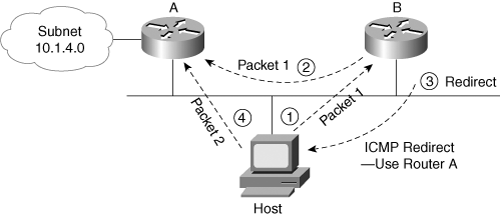
\includegraphics[width = 0.8\linewidth]{img/4/data-plane/ICMP-redirect.png}
    \caption{ICMP redirect}
    \label{fig:icmp-redirect}
\end{figure}

%//==============================--@--==============================//%